\documentclass[tikz,border=2pt]{standalone}
\usepackage{amsmath}\usepackage{pgfplots}\usepgfplotslibrary{groupplots}\pgfplotsset{compat=1.18}
\definecolor{cA}{HTML}{2166AC}\definecolor{cB}{HTML}{1B9E77}\definecolor{cC}{HTML}{D95F02}\definecolor{cD}{HTML}{C51B7D}\definecolor{cE}{HTML}{7570B3}
\begin{document}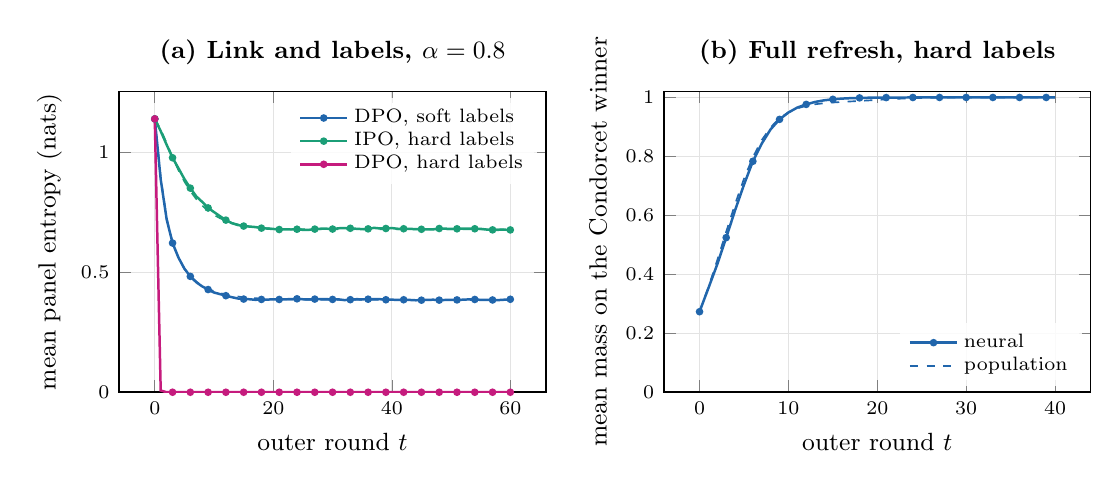
\begin{tikzpicture}
\begin{groupplot}[group style={group size=2 by 1, horizontal sep=1.5cm}, width=7.0cm, height=5.4cm, tick label style={font=\scriptsize}, label style={font=\small}, title style={font=\small\bfseries}, grid=major, grid style={draw=gray!22, line width=0.25pt}, axis line style={black, line width=0.6pt}, legend style={font=\scriptsize, draw=none, fill=white, fill opacity=0.85, text opacity=1, cells={anchor=west}, row sep=-2pt}]
\nextgroupplot[title={(a) Link and labels, $\alpha=0.8$}, xlabel={outer round $t$}, ylabel={mean panel entropy (nats)}, ymin=0, legend style={at={(0.98,0.98)}, anchor=north east}]
\addplot[cA, line width=0.9pt, mark=*, mark size=0.9pt, mark repeat=3] coordinates {(0,1.1396) (1,0.88779) (2,0.72177) (3,0.62204) (4,0.56125) (5,0.5152) (6,0.48302) (7,0.45868) (8,0.44135) (9,0.42812) (10,0.41572) (11,0.40913) (12,0.40258) (13,0.39631) (14,0.39086) (15,0.3884) (16,0.38765) (17,0.38528) (18,0.38696) (19,0.38625) (20,0.38741) (21,0.38677) (22,0.38727) (23,0.38829) (24,0.38952) (25,0.3876) (26,0.38706) (27,0.38829) (28,0.38845) (29,0.38799) (30,0.38698) (31,0.38729) (32,0.38417) (33,0.38586) (34,0.38781) (35,0.3875) (36,0.38797) (37,0.38838) (38,0.38794) (39,0.3856) (40,0.38579) (41,0.38522) (42,0.38558) (43,0.3848) (44,0.38345) (45,0.38381) (46,0.38505) (47,0.3858) (48,0.38401) (49,0.38464) (50,0.38482) (51,0.38499) (52,0.38575) (53,0.38712) (54,0.38679) (55,0.38519) (56,0.38545) (57,0.38467) (58,0.38418) (59,0.38581) (60,0.38765)}; \addlegendentry{DPO, soft labels}
\addplot[cA, dashed, line width=0.6pt, forget plot] coordinates {(0,1.1396) (1,0.89665) (2,0.72543) (3,0.62478) (4,0.55993) (5,0.51568) (6,0.48426) (7,0.46129) (8,0.44416) (9,0.43117) (10,0.42121) (11,0.41351) (12,0.40751) (13,0.40281) (14,0.39911) (15,0.39619) (16,0.39388) (17,0.39204) (18,0.39059) (19,0.38943) (20,0.3885) (21,0.38777) (22,0.38718) (23,0.38671) (24,0.38634) (25,0.38604) (26,0.3858) (27,0.38561) (28,0.38545) (29,0.38533) (30,0.38523) (31,0.38515) (32,0.38509) (33,0.38504) (34,0.385) (35,0.38497) (36,0.38495) (37,0.38492) (38,0.38491) (39,0.3849) (40,0.38488) (41,0.38488) (42,0.38487) (43,0.38486) (44,0.38486) (45,0.38486) (46,0.38485) (47,0.38485) (48,0.38485) (49,0.38485) (50,0.38485) (51,0.38485) (52,0.38485) (53,0.38485) (54,0.38484) (55,0.38484) (56,0.38484) (57,0.38484) (58,0.38484) (59,0.38484) (60,0.38484)};
\addplot[cB, line width=0.9pt, mark=*, mark size=0.9pt, mark repeat=3] coordinates {(0,1.1396) (1,1.0887) (2,1.0321) (3,0.97765) (4,0.93372) (5,0.88889) (6,0.85102) (7,0.81665) (8,0.79372) (9,0.76846) (10,0.7511) (11,0.73411) (12,0.71763) (13,0.70492) (14,0.69733) (15,0.69281) (16,0.69062) (17,0.6886) (18,0.68417) (19,0.68231) (20,0.68078) (21,0.67833) (22,0.67917) (23,0.67846) (24,0.67966) (25,0.67698) (26,0.67704) (27,0.68008) (28,0.68169) (29,0.68184) (30,0.68034) (31,0.68355) (32,0.68471) (33,0.68357) (34,0.6815) (35,0.68011) (36,0.68115) (37,0.68539) (38,0.68282) (39,0.68268) (40,0.68446) (41,0.68151) (42,0.68164) (43,0.68111) (44,0.68008) (45,0.67941) (46,0.6786) (47,0.67929) (48,0.68263) (49,0.68185) (50,0.68113) (51,0.68145) (52,0.68252) (53,0.68228) (54,0.68156) (55,0.68109) (56,0.67827) (57,0.67697) (58,0.67741) (59,0.6777) (60,0.67671)}; \addlegendentry{IPO, hard labels}
\addplot[cB, dashed, line width=0.6pt, forget plot] coordinates {(0,1.1396) (1,1.0965) (2,1.0388) (3,0.97989) (4,0.92575) (5,0.87851) (6,0.83856) (7,0.80547) (8,0.77847) (9,0.75671) (10,0.73932) (11,0.72555) (12,0.71472) (13,0.70625) (14,0.69968) (15,0.69459) (16,0.69069) (17,0.68771) (18,0.68545) (19,0.68374) (20,0.68246) (21,0.68151) (22,0.6808) (23,0.68029) (24,0.67992) (25,0.67965) (26,0.67946) (27,0.67933) (28,0.67925) (29,0.67919) (30,0.67915) (31,0.67913) (32,0.67912) (33,0.67912) (34,0.67912) (35,0.67912) (36,0.67913) (37,0.67913) (38,0.67914) (39,0.67915) (40,0.67915) (41,0.67916) (42,0.67916) (43,0.67916) (44,0.67917) (45,0.67917) (46,0.67917) (47,0.67917) (48,0.67917) (49,0.67918) (50,0.67918) (51,0.67918) (52,0.67918) (53,0.67918) (54,0.67918) (55,0.67918) (56,0.67918) (57,0.67918) (58,0.67918) (59,0.67918) (60,0.67918)};
\addplot[cD, line width=0.9pt, mark=*, mark size=0.9pt, mark repeat=3] coordinates {(0,1.1396) (1,0.0073086) (2,2.8293e-07) (3,3.904e-10) (4,7.6757e-13) (5,6.9634e-16) (6,2.0599e-17) (7,1.0058e-18) (8,9.9389e-21) (9,7.752e-22) (10,6.4638e-23) (11,6.2511e-23) (12,5.0326e-24) (13,9.8778e-24) (14,5.2545e-24) (15,1.422e-23) (16,7.9374e-24) (17,1.1599e-23) (18,2.9614e-25) (19,1.888e-23) (20,1.9949e-26) (21,1.7228e-24) (22,2.0685e-27) (23,2.1793e-27) (24,5.7564e-26) (25,5.6176e-25) (26,3.7854e-25) (27,2.3647e-26) (28,7.1001e-26) (29,1.3114e-28) (30,4.7966e-28) (31,1.1565e-27) (32,9.6074e-30) (33,1.8074e-29) (34,8.1572e-28) (35,1.0499e-28) (36,2.2968e-30) (37,1.836e-28) (38,2.098e-30) (39,2.1856e-30) (40,3.4082e-33) (41,1.938e-33) (42,1.9384e-30) (43,8.6597e-29) (44,2.5172e-30) (45,1.0522e-29) (46,9.3029e-30) (47,1.0048e-29) (48,8.7877e-32) (49,5.6776e-33) (50,4.3476e-31) (51,4.9171e-28) (52,3.5805e-41) (53,1.5644e-37) (54,2.2809e-37) (55,1.4415e-38) (56,1.1056e-38) (57,6.5397e-39) (58,2.1354e-38) (59,4.4698e-40) (60,3.4826e-41)}; \addlegendentry{DPO, hard labels}
\nextgroupplot[title={(b) Full refresh, hard labels}, xlabel={outer round $t$}, ylabel={mean mass on the Condorcet winner}, ymin=0, ymax=1.02, legend style={at={(0.98,0.02)}, anchor=south east}]
\addplot[cA, line width=0.9pt, mark=*, mark size=0.9pt, mark repeat=3] coordinates {(0,0.27321) (1,0.35334) (2,0.43455) (3,0.52456) (4,0.61749) (5,0.70418) (6,0.78342) (7,0.84365) (8,0.892) (9,0.9257) (10,0.94896) (11,0.96578) (12,0.97647) (13,0.98481) (14,0.99033) (15,0.99372) (16,0.99614) (17,0.99765) (18,0.99851) (19,0.99911) (20,0.99946) (21,0.99967) (22,0.99979) (23,0.99988) (24,0.99993) (25,0.99996) (26,0.99997) (27,0.99998) (28,0.99999) (29,0.99999) (30,1) (31,1) (32,1) (33,1) (34,1) (35,1) (36,1) (37,1) (38,1) (39,1) (40,1)}; \addlegendentry{neural}
\addplot[cA, dashed, line width=0.6pt] coordinates {(0,0.27321) (1,0.3565) (2,0.44865) (3,0.54462) (4,0.63841) (5,0.72415) (6,0.79729) (7,0.85547) (8,0.8988) (9,0.92925) (10,0.9497) (11,0.963) (12,0.97149) (13,0.97691) (14,0.98044) (15,0.98289) (16,0.98479) (17,0.98648) (18,0.98816) (19,0.98991) (20,0.9917) (21,0.99346) (22,0.99509) (23,0.99648) (24,0.99759) (25,0.99841) (26,0.99898) (27,0.99936) (28,0.9996) (29,0.99976) (30,0.99985) (31,0.99991) (32,0.99994) (33,0.99997) (34,0.99998) (35,0.99999) (36,0.99999) (37,1) (38,1) (39,1) (40,1)}; \addlegendentry{population}
\end{groupplot}
\end{tikzpicture}\end{document}
